%==============================================================================
% Document Header
%==============================================================================
\documentclass[a4paper,11pt]{article}

% Color package
\usepackage[usenames,dvipsnames,table]{xcolor}

% Hyperrefs
\usepackage[
  colorlinks = true,
  linkcolor  = Mahogany,
  citecolor  = Mahogany,
  urlcolor   = blue,
]{hyperref}

% Longtable
\usepackage{longtable}

% Graphics, multirow
\usepackage{graphicx}
\usepackage{multirow}

% Appendix package
\usepackage[toc,page]{appendix}

% Listings package
\usepackage{listings}


\usepackage{fancyhdr}
\setlength{\headheight}{15.2pt}
\pagestyle{fancy}
\fancyhead[L]{\nouppercase{\leftmark}}
\fancyhead[R]{}
\renewcommand{\footrulewidth}{0.4pt}

% Row number command
\newcounter{rownr}
\newcommand{\rownumber}{\stepcounter{rownr}\arabic{rownr}}

%==============================================================================
% Start of document
%==============================================================================
\begin{document}

%------------------------------------------------------------------------------
% Title
%------------------------------------------------------------------------------
\begin{titlepage}

\vspace*{3cm}

\noindent{\LARGE \textbf{I$^2$C Slave Core}}

\noindent \rule{\textwidth}{.1cm}

\hfill\today

\vspace*{3cm}

\begin{figure}[h]
  
\includegraphics[height=3cm]{fig/cern-logo}
  \hfill
  
\includegraphics[height=3cm]{fig/ohwr-logo}
\end{figure}

\vfill

\noindent {\Large \textbf{Theodor-Adrian Stana (CERN/BE-CO-HT)}}

\noindent \rule{\textwidth}{.05cm}

\end{titlepage}


%------------------------------------------------------------------------------
% Revision history
%------------------------------------------------------------------------------
\thispagestyle{empty}
\section*{Revision history}

\centerline
{
  \rowcolors{2}{white}{gray!25}
  \begin{tabular}{l c p{.6\textwidth}}
  \hline
  \multicolumn{1}{c}{\textbf{Date}} & \multicolumn{1}{c}{\textbf{Version}} & \multicolumn{1}{c}{\textbf{Change}} \\
  \hline
  28-10-2013 & 0.1 & First draft \\
  18-12-2013 & 1.0 & Added WDTO bit to status register and information about the FSM watchdog
                     mechanism \\
  13-02-2014 & 1.1 & Made memory map prettier \\
  \hline
  \end{tabular}
}

\pagebreak
\pagenumbering{roman}
\setcounter{page}{1}
\tableofcontents

%------------------------------------------------------------------------------
% List of figs, tables
%------------------------------------------------------------------------------
\pagebreak
\listoffigures
\listoftables

%------------------------------------------------------------------------------
% List of abbreviations
%------------------------------------------------------------------------------
\pagebreak
\section*{List of Abbreviations}
\begin{tabular}{l l}
FPGA  & Field-Programmable Gate Array \\
ICAP  & Internal Configuration Access Port \\
IPROG & Internal PROGRAM\_B \\
OHWR  & Open Hardware Repository \\
PROM  & Programmable Read-Only Memory \\
SPI   & Serial Peripheral Interface \\
\end{tabular}

\pagebreak
\pagenumbering{arabic}
\setcounter{page}{1}

%==============================================================================
% SEC: Intro
%==============================================================================
\section{Introduction}
\label{sec:intro}

Xilinx MultiBoot technology~\cite{ug380} allows reprogramming an FPGA by downloading a
bitstream to a PROM chip external to the FPGA and then issuing an IPROG (Internal
PROGRAM\_B) command to the configuration logic of the FPGA. This command triggers
deletion of the FPGA configuration and rewriting it with the new configuration
written to the PROM.

This document describes \textit{wb\_xil\_multiboot}, an Open Hardware~\cite{ohwr}
FPGA design that can be used to remotely reprogram a Xilinx Spartan-6 FPGA using
MultiBoot technology. The core can be found within the \textit{general-cores}
library~\cite{gencores-ohwr} on OHWR.

\begin{figure}[h]
  \centerline{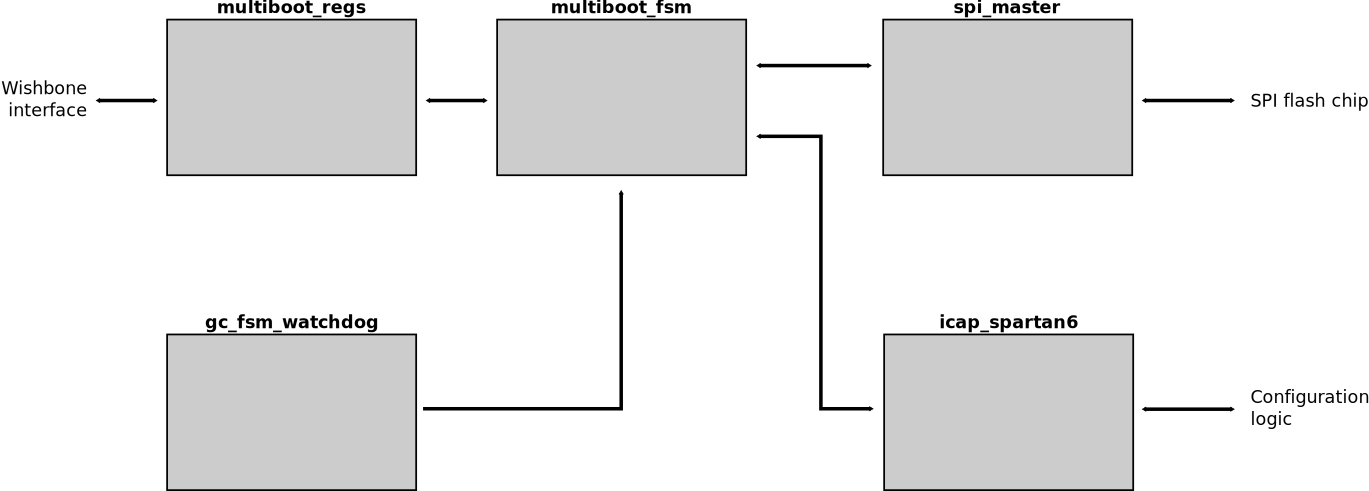
\includegraphics[width=\textwidth]{fig/multiboot-bd}}
  \label{fig:multiboot-bd}
  \caption{Block diagram of \textit{wb\_xil\_multiboot} module}
\end{figure}

The main features of the \textit{wb\_xil\_multiboot} module are:
\begin{itemize}
  \item software controls operation of the module
  \begin{itemize}
    \item Wishbone interface implements registers for control and status readout
    \item writing FPGA bitstream data to the flash chip
    \item issuing reprogramming command to the FPGA (via Xilinx ICAP)
    \item reading boot status register from the FPGA configuration logic (via Xilinx ICAP)
  \end{itemize}
  \item a finite-state machine (FSM) controls writing to the flash chip and sending the
  reprogramming command to the FPGA
  \item modular, easily modifiable design
  \begin{itemize}
    \item PROM chip is controlled by software, so virtually any 8-bit SPI PROM chip is
    supported by writing software to send the various commands to the chip
    \item Wishbone interface can easily be replaced by some other interconnect (e.g., AXI)
  \end{itemize}
\end{itemize}

A block diagram of the \textit{wb\_xil\_multiboot} module is shown in Figure~\ref{fig:multiboot-bd}.
Users can write bitstream data to a flash by writing each byte of the bitstream to a module register
(in the \textit{multiboot\_regs}) module. Writing to the flash is done via the \textit{spi\_master}
module under the control of the finite-state machine (FSM) module (\textit{multiboot\_fsm}). After the
bitstream has been written to the flash module, a remote reprogramming command is sent
to the configuration logic by setting a bit in one of the control registers. The
Xilinx \textit{ICAP\_SPARTAN6} primitive is the interface between the \textit{wb\_xil\_multiboot}
module and the FPGA configuration logic.

For the rest of the document, the external PROM chip that the FPGA uses to
program itself will be referred to as flash, since a flash chip was used
as the external PROM during the design of the module. However, this does not
mean \textit{wb\_xil\_multiboot} works only with flash chips. Any 8-bit SPI PROM
should be usable with the \textit{wb\_xil\_multiboot} design.

%==============================================================================
% SEC: Instantiation
%==============================================================================
\section{Instantiation}
\label{sec:instantiation}

Table~\ref{tbl:ports} lists the ports of the \textit{wb\_xil\_multiboot} module.
In order to instantiate the MultiBoot module, one needs to connect
the Wishbone slave ports to a Wishbone master, such as the \textit{xwb\_crossbar}
Wishbone crossbar module on OHWR \cite{gencores-ohwr}. The SPI ports should be
connected directly to the FPGA output ports connected to the flash chip.

\begin{table}[h]
  \caption{Ports of the Xilinx MultiBoot module}
  \label{tbl:ports}
  \centerline
  {
    \rowcolors{2}{white}{gray!25}
    \begin{tabular}{l p{.6\textwidth}}
    \hline
    \multicolumn{1}{c}{\textbf{Port}} & \multicolumn{1}{c}{\textbf{Description}} \\
    \hline
    clk\_i        & Clock input (max. 20~MHz) \\
    rst\_n\_i     & Active-low reset input \\
    wbs\_i        & Wishbone slave interface inputs \\
    wbs\_o        & Wishbone slave interface outputs \\
    spi\_cs\_n\_o & Active-low chip select output \\
    spi\_sclk\_o  & SPI clock output \\
    spi\_mosi\_o  & SPI data output line (Master Out, Serial In) \\
    spi\_miso\_i  & SPI data input line (Master In, Serial Out) \\
    \hline
    \end{tabular}
  }
\end{table}

Note that in order to use the module, the OHWR \textit{general-cores}
library~\cite{gencores-ohwr} needs to be imported into the design. This library is where
the structures for the Wishbone slave interface ports (\textit{wbs\_i} and \textit{wbs\_o})
are defined.

Further note that the maximum \textit{clk\_i} frequency allowable is 20~MHz, due
to constraints of the ICAP component from Xilinx. Should a greater system clock
frequency be used in the design, the user can instantiate the \textit{wb\_xil\_multiboot}
module using a \textit{wb\_clock\_crossing} component from the OHWR \textit{general-cores}
library~\cite{gencores-ohwr}. This is shown in Figure~\ref{fig:inst-clkcross}.

\begin{figure}
  \centerline{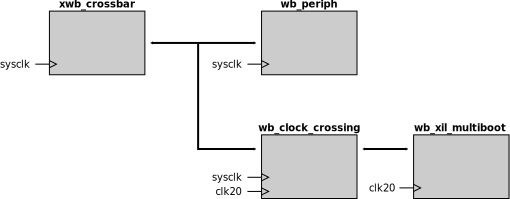
\includegraphics[width=\textwidth]{fig/inst-clkcross}}
  \caption{Instantiation when the system clock is greater than 20~MHz}
  \label{fig:inst-clkcross}
\end{figure}

%==============================================================================
% SEC: Using
%==============================================================================
\pagebreak
\section{Using the Xilinx MultiBoot module}
\label{sec:instantiation}

For an example project of where the Xilinx MultiBoot module is used, see the
CONV-TTL-BLO project~\cite{ctb-proj}. The firmware of this projectuses the MultiBoot
module. The project also contains example Python scripts for writing a bitstream to
the flash. Refer to the project webpage~\cite{ctb-proj} for more information.

Table~\ref{tbl:workflow} shows the MultiBoot workflow~\cite{xtp059}. See \cite{gen-bitstream}
for pointers on how to generate a MultiBoot bitstream. The address map of the MultiBoot module
can be found in Appendix~\ref{app:memmap}. This appendix details the various registers the
user should write as part of the MultiBoot workflow.

\setcounter{rownr}{0}

\begin{table}[h]
  \caption{MultiBoot workflow}
  \label{tbl:workflow}
  \centerline {
    \rowcolors{2}{white}{gray!25}
    \begin{tabular}{c p{.7\textwidth}}
    \hline
    \textbf{Step} & \multicolumn{1}{c}{\textbf{Action}} \\
    \hline
    \rownumber & Prepare a Xilinx FPGA bitstream                                         \\
    \rownumber & Send the bitstream to the flash by writing to the FAR register          \\
    \rownumber & Write the MultiBoot bitstream start address and flash chip read command
                 op-code into the MBBAR register                                         \\
    \rownumber & Write the Golden bitstream start address and flash chip read command
                 op-code into the GBBAR register                                         \\
    \rownumber & Unlock the IPROG bit in the FPGA by setting CR.IPROG\_UNLOCK            \\
    \rownumber & Issue a reprogramming command to the FPGA by setting CR.IPROG           \\
    \hline
    \end{tabular}
  }
\end{table}


%==============================================================================
% SEC: MultiBoot
%==============================================================================
\section{Xilinx MultiBoot technology}
\label{sec:multiboot}

Spartan-6 configuration logic is organized in a set of frames, which can be written to
or read from using 16-bit word transfers. A Spartan-6 FPGA bitstream consists of
commands that access the FPGA configuration logic to read and write these frames,
as well as the data for the configuration logic frames.

When using the MultiBoot technology, multiple bitstreams exist for one FPGA.
These bitstreams are all stored on the attached flash chip and the user can
send a special instruction called IPROG (Internal PROGRAM\_B) to reprogram the
FPGA chip using one of the bitstreams on the flash.

Most MultiBoot designs will contain at least three bitstreams, as shown in
Figure~\ref{fig:multiboot}. When the FPGA board is powered on, if it is configured
in master mode configuration~\cite{ug380}, the FPGA will start loading a bitstream
from address zero of the attached flash chip. This is where the Header bitstream
resides. This small bitstream contains a synchronization word for the configuration
logic, sets the start address of the MultiBoot and Golden bitstreams and sends
an IPROG command to the configuration logic.

\begin{figure}
  \centerline{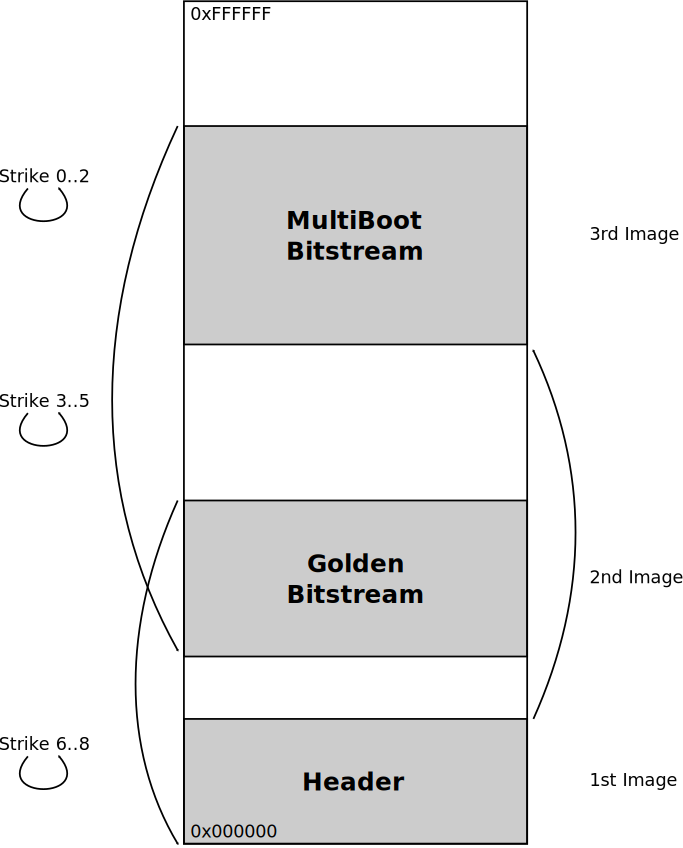
\includegraphics[scale=.45]{fig/multiboot}}
  \label{fig:multiboot}
  \caption{Bitstreams in a MultiBoot design}
\end{figure}

The IPROG command causes the configuration logic to start loading the MultiBoot 
bitstream from the flash chip, starting at the given MultiBoot address. If the MultiBoot
bitstream fails to load three times (see below for bitstream load failure reasons),
the configuration logic falls back to the Golden bitstream. This is a bitstream
which is known to be safe, should the MultiBoot bitstream be corrupted on load.

Should the Golden bitstream also be corrupted, the configuration logic
tries to load it three times and then returns to the Header bitstream. When here,
the configuration logic attempts to load the MultiBoot and Golden bitstreams three
more times, before configuration failure.

A strike counter is used to select between which of the three bitstreams is loaded.
This strike counter is stored in the configuration BOOTSTS register and can only be
reset by a power-on reset or by pulsing the FPGA's PROGRAM\_B pin. The strike counter
is shared among the three bitsreams; as Figure~\ref{fig:multiboot} shows and as just
described, each bitstream is selected based on the value of this counter:

\begin{itemize}
  \item if it is 0..2, the MultiBoot bitstream gets loaded
  \item if it is 3..5, the Golden bitstream gets loaded
  \item if it is 6..8, the Header bitstream gets loaded, and MultiBoot and Golden
  bitstreams are attempted three more times
  \item if it is 9, configuration is halted
\end{itemize}

%------------------------------------------------------------------------------
\subsection{Reasons for bitstream load failure}

There are two ways in which a bitstream load can fail:
\begin{itemize}
  \item synchronization word Watchdog timeout
  \item bitstream CRC error
\end{itemize}

Prior to performing any work, the FPGA configuration logic looks for a synchronization word
in the bitstream. This synchronization word is shown in Table~\ref{tbl:sync-word}. The
configuration logic contains a Watchdog timer that counts down from a value specified by
the Xilinx \textit{bitgen} tool when the bitstream is generated (see Table~\ref{tbl:bitgen}).
The Watchdog is disabled when the synchronization word is found. If the Watchdog timer
times out, the strike count is incremented and configuration is reattempted as described above.

Note that the Watchdog timer is only enabled in master configuration modes, when
configuration restarts. It is disabled when the synchronization word is found,
or when the FPGA uses one of the other configuration modes~\cite{ug380}.

\begin{table}[h]
  \label{tbl:sync-word}
  \caption{Bitstream synchronization word}
  \centerline {
  \rowcolors{2}{white}{gray!25}
  \begin{tabular}{c c c c}
    \hline
    \textbf{31 .. 24} & \textbf{23..16} & \textbf{15..8} & \textbf{7..0} \\
    \hline
    0xAA & 0x99 & 0x55 & 0x66 \\
    \hline
  \end{tabular}
  }
\end{table}

The second failure mode of the configuration is based on the bitstream CRC. Each
bitstream contains at the end a CRC word which the configuration logic checks
before putting the FPGA in running mode. If the CRC at the end of the bitstream
does not correspond to what the configuration logic computes, a CRC error occurs
and the strike count is incremented as described above.

\begin{table}[h]
  \label{tbl:bitgen}
  \caption{\textit{bitgen} flags}
  \centerline {
  \rowcolors{2}{white}{gray!25}
  \begin{tabular}{l l p{.6\textwidth}}
    \hline
    \multicolumn{1}{c}{\textbf{Flag}} & \multicolumn{1}{c}{\textbf{Setting}} & \multicolumn{1}{c}{\textbf{Description}} \\
    \hline
    -g reset\_on\_err & Yes    & Enables the strike count mechanism for retrying to load
                               the bitstream \\
    -g CRC          & Enable & Enables the generation of a CRC at the end of the bitstream \\
    -g TIMER\_CFG   & 1fff   & Sets the watchdog timeout value to 8191 CCLK cycles \\
    \hline
  \end{tabular}
  }
\end{table}

For configuration to be reattempted and to be able to generate configuration
errors, the configuration logic needs some information present in the bitstream.
This information can be provided by setting some \textit{bitgen} flags when
generating the bitstream. The necessary flags with the recommended settings
are listed in Table~\ref{tbl:bitgen}. For more information on \textit{bitgen}
and these flags, refer to \cite{xil-devref}.

%------------------------------------------------------------------------------
\subsection{Generating the bitstreams}

Refer to \cite{gen-bitstream} for information on how to generate the various
bitstreams for a MultiBoot design.

%------------------------------------------------------------------------------
\subsection{Important note regarding MultiBoot bitstreams}

Users should be aware that they should include the \textit{wb\_xil\_multiboot} module
when generating a new MultiBoot bitsream. Otherwise, once a bitstream without
the \textit{wb\_xil\_multiboot} module inside it is loaded into the FPGA, the
remote reprogramming capability of the FPGA is lost, and the user will need
to use JTAG or other means to program the FPGA with a MultiBoot-enabled design.

Thus, always remember to include the \textit{wb\_xil\_multiboot} module in any bitstream
generated after the Golden bitstream.

%==============================================================================
% SEC: Implementation
%==============================================================================
\section{Implementation}
\label{sec:implem}

A block diagram of the design has already been presented in
Figure~\ref{fig:multiboot-bd}. This section describes the actions of the sub-modules
in the \textit{wb\_xil\_multiboot} module. The description is rather high-level,
some details are omitted for ease of understanding. The main purpose of this
section is for the reader to understand how the MultiBoot module works together with
the flash chip and the configuration logic to achieve FPGA reprogramming, rather
than specifying every detail about the module and its sub-modules. For more involved
details, the user is free to consult the code in the project
repository~\cite{gencores-ohwr}.

\begin{figure}[h]
  \centerline{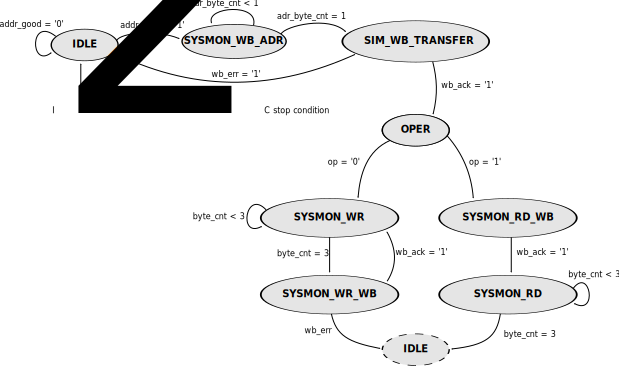
\includegraphics[width=.9\textwidth]{fig/fsm}}
  \caption{Phases of the \textit{multiboot\_fsm}}
  \label{fig:fsm}
\end{figure}

\begin{table}[h]
  \caption{Phases of the \textit{multiboot\_fsm}}
  \label{tbl:fsm}
  \centerline {
    \rowcolors{2}{white}{gray!25}
    \begin{tabular}{p{.185\textwidth} p{.7\textwidth}}
    \hline
    \multicolumn{1}{c}{\textbf{Phase}} & \multicolumn{1}{c}{\textbf{Description}} \\
    \hline
    \textbf{IDLE}         & Wait for one of the following control bits to be set: \newline
                            CR.RDCFGREG \newline
                            CR.IPROG \newline
                            FAR.XFER \\
    \textbf{SPI transfer} & Shift out NBYTES of the three DATA fields in the FAR register,
                            and simultaneously shift in data received from the flash \newline
                            When NBYTES have been sent, FAR.READY is written high and
                            the FSM returns to IDLE \\
    \textbf{IPROG}        & IPROG sequence (Table 7-1, p.130~\cite{ug380}) \\
    \textbf{Read status register} & Configuration register readout sequence (Table 6-1, p.113~\cite{ug380}) \\
    \hline
    \end{tabular}
  }
\end{table}

The \textit{multiboot\_fsm} module is at the heart of the design. It implements
a finite-state machine (FSM) with 34 states, which controls operation of the module.
A simplified diagram of the FSM is shown in Figure~\ref{fig:fsm}. The diagram shows the various
phases the FSM is in, and Table~\ref{tbl:fsm} lists these phases. Bear in mind
that each phase may contain multiple FSM states. However, many of these states
are just steps of accessing configuration logic through the Xilinx ICAP module,
so for simplicity they are not listed in this manual. Refer to the code for
more complete description.

%------------------------------------------------------------------------------
\subsection{Sending data to the flash chip}
\label{sec:implem-spi}

Table~\ref{tbl:data-seq} summarizes the flash read and write sequence. A more verbose
description is offered below.

\setcounter{rownr}{0}

\begin{table}[h]
  \caption{Flash data sequence}
  \label{tbl:data-seq}
  \centerline{
    \rowcolors{2}{white}{gray!25}
  \begin{tabular}{c p{.7\textwidth}}
    \hline
    \textbf{Step} & \multicolumn{1}{c}{\textbf{Action}} \\
    \hline
    \rownumber & User sets FAR.NBYTES to the number of data bytes to write \\
    \rownumber & User writes NBYTES FAR.DATA fields with the data to send to the flash \\
    \rownumber & User sets FAR.CS to '1' for a transfer with the flash chip enabled, or
                 to '0' for a dummy transfer (e.g., wait interval between flash commands,
                 with the chip select high) \\
    \rownumber & User sets FAR.XFER to '1' to start the SPI transfer \newline
                 (FAR.XFER is automatically cleared by hardware) \\
    \rownumber & The \textit{multiboot\_fsm} starts shifting out NBYTES DATA fields
                 to the \textit{spi\_master}, starting with DATA[0] \\
    \rownumber & The \textit{spi\_master} handles shifting out each bit in a byte \\
    \rownumber & When done, the \textit{spi\_master} signals the \textit{multiboot\_fsm},
                 which shifts out the next byte (if NBYTES $>$ 0) \\
    \rownumber & When NBYTES bytes have been shifted out, the \textit{multiboot\_fsm}
                 sets the FAR.READY bit \\
    \rownumber & After FAR.READY is set, NBYTES DATA fields contain data retrieved from
                 the flash \\
    \hline
  \end{tabular}
  }
\end{table}

Data to be sent to the flash chip is written in the FAR (see Appendix~\ref{app:memmap-far}).
Up to three data bytes can be sent via the FAR during one transfer phase. These data
bytes are written in the DATA fields in little-endian order. The NBYTES field selects
how many of the DATA fields contain bytes to send. Setting XFER to '1' with CS set to
'1' starts the transfer. Setting XFER to '1' with CS set to '0' starts a dummy
transfer, with the flash chip not selected.

The transfer is performed via the \textit{spi\_master} module, which handles the
shifting of each DATA byte to the flash. However, the \textit{spi\_master} module
can only send one byte at a time, so the \textit{multiboot\_fsm} module handles
shifting bytes to the \textit{spi\_master}. After a byte has been transferred
between the FPGA and the flash, the \textit{multiboot\_fsm} places the byte
returned from the flash into the DATA byte that has just been sent. For example,
after sending DATA[0], the byte received from the flash is placed into DATA[0];
after sending DATA[1], the byte received from the flash is placed into DATA[1].

When NBYTES data transfers have been completed, the \textit{multiboot\_fsm} sets
the signal for the FAR.READY bit to '1', to signal a completed transfer. The user
can now read the DATA fields for data retrieved from the flash.

The feature of using more than one DATA field in the FAR is useful when a lower-speed
interface than SPI is used to access the FAR register (e.g., the VBCP interface in
the CONV-TTL-BLO project~\cite{ctb-proj}). If the interface used to access the FAR
is fast, only one byte in the FAR register may be used, and NBYTES left to 0.

Appendix~\ref{app:multiple-spi} gives an example of how data can be written to flash.

The following settings are used for the SPI communication (Figure~\ref{fig:spi-mode}).
\begin{itemize}
  \item CPOL = 0
  \item CPHA = 0
\end{itemize}

\begin{figure}[h]
  \centerline{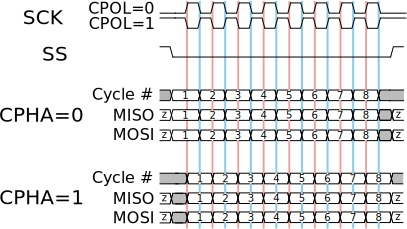
\includegraphics[width=.7\textwidth]{fig/spi-mode}}
  \caption{SPI settings (source: Wikipedia)}
  \label{fig:spi-mode}
\end{figure}

This yields that data bits are shifted out from the FPGA on the falling edge of SCLK
and shifted in from the flash chip on the rising edge of SCLK.

%------------------------------------------------------------------------------
\subsection{Reading FPGA configuration registers}
\label{sec:implem-rdcfgreg}

The Spartan-6 FPGA contains registers which can be read to get the stauts of the
configuration logic. In order to read these registers, a special sequence must be
followed. The sequece (listed in Table 6-1 of~\cite{ug380}) is implemented in the
\textit{multiboot\_fsm}. Table~\ref{tbl:rdcfgreg-seq} lists the sequence users
should follow to read out an FPGA configuration register via the \textit{wb\_xil\_multiboot}
module.

\setcounter{rownr}{0}

\begin{table}[h]
  \caption{Configuration register readout via \textit{wb\_xil\_multiboot}}
  \label{tbl:rdcfgreg-seq}
  \centerline {
    \rowcolors{2}{white}{gray!25}
    \begin{tabular}{c p{.7\textwidth}}
    \hline
    \multicolumn{1}{c}{\textbf{Step}} & \multicolumn{1}{c}{\textbf{Action}} \\
    \hline
    \rownumber & User writes the FPGA configuration register address (Table 5-30, p.94~\cite{ug380})
                 in the CFGREGADR field of the CR \\
    \rownumber & User sets the CR.RDCFGREG bit to '1' to initiate a configuration register
                 read via the ICAP module \newline
                 (CR.RDCFGREG is automatically cleared by hardware) \\
    \rownumber & The \textit{multiboot\_fsm} performs the sequence in Table 6-1, p.113~\cite{ug380}
                 and returns one 16-bit value of the configuration register to the CFGREGIMG
                 field of IMGR and sets the VALID bit of the same register to '1' \\
    \rownumber & The user reads the configuration register value from IMGR.CFGREGIMG if the
                 VALID bit is '1' \\
    \hline
    \end{tabular}
  }
\end{table}

When the user sets the RDCFGREG bit in the \textit{wb\_xil\_multiboot} control register (CR),
the \textit{multiboot\_fsm} initiates the configuration register readout sequence.
It first sends a synchronization word, and then takes the value of CFGREGADR from
the CR and use it to build a Type 1 configuration frame to read the configuration
register (see~\cite{ug380}, p.~93 for more details). The configuration logic will
respond to this frame with the value of the configuration register. This value is
placed in the CFGREGIMG field of the image register, and the \textit{multiboot\_fsm}
continues to perform the final steps of the configuration register readout sequence,
prior to returning to IDLE.

Note that some configuration registers in the Spartan-6 FPGA are more than 16 bits wide.
The \textit{wb\_xil\_multiboot} module does not support reading the full length of the
registers; it can only return the least significant 16 bits of the registers.

%------------------------------------------------------------------------------
\subsection{Sending the IPROG command}

Table~\ref{tbl:iprog} lists the actions needed to issue the IPROG command to the
FPGA using the \textit{wb\_xil\_multiboot} module. When the IPROG bit is set in the CR,
the \textit{multiboot\_fsm} handles sending the IPROG sequence (Table 7-1,
p.130~\cite{ug380}) to the ICAP.

\setcounter{rownr}{0}

\begin{table}[h]
  \caption{Sequence for sending the IPROG command}
  \label{tbl:iprog}
  \centerline {
    \rowcolors{2}{white}{gray!25}
    \begin{tabular}{c p{.7\textwidth}}
    \hline
    \textbf{Step} & \multicolumn{1}{c}{\textbf{Action}} \\
    \hline
    \rownumber & User sends the bitstream to the flash chip (Section~\ref{sec:implem-spi}) \\
    \rownumber & User sets the IPROG\_UNL bit in the CR \\
    \rownumber & User sets the IPROG bit in the CR \\
    \rownumber & The \textit{multiboot\_fsm} performs the sequence in Table 7-1, p.130~\cite{ug380}
                 and sends the IPROG command \\
    \rownumber & The FPGA starts deleting the configuration logic and loading the
                 new bitstream from the flash \\
    \rownumber & After configuration finishes, the user reads the custom firmware
                 version number register to see that the reprogramming was successful \\
    \hline
    \end{tabular}
  }
\end{table}

Note that after the IPROG command is sent, the FPGA starts the reconfiguration
sequence and communication to it will be lost until the new bitstream is loaded
is sent.

The user should implement some form of firmware version numbering to detect whether
an IPROG succeeds. This version number can be stored into a read-only register in the
FPGA and read after the IPROG command. An example of this is given in the CONV-TTL-BLO
project~\cite{ctb-proj}.

%------------------------------------------------------------------------------
\subsection{FSM watchdog timer}

An FSM watchdog timer component (\textit{gc\_fsm\_watchdog} on OHWR) is instantiated
in the design. This component is used to reset the main FSM in case an error
occurs and the FSM stalls waiting for an action. The timeout value of the
watchdog timer is set to 512, since it was established from the component's
simulation that the phase of the FSM that would take the longest number of
cycles to complete (the SPI phase) would complete and return to IDLE
within 218 clock cycles. A safe value of 512 was selected to allow some tolerance
to the FSM, while making sure that it would return to its IDLE state in
case of errors.

When the FSM watchdog fires, the SR.WDTO bit is set. This bit can be cleared by
writing a '1' to it.

%==============================================================================
% SEC: Modifying
%==============================================================================
\section{Modifying the design}
\label{sec:modify}

The \textit{wb\_xil\_multiboot} module is purposely modular in case users want to
interface to different FPGA interconnect standards, or different flash chips.
In order to make modifications to the design, knowledge of VHDL is required.

If the user would like to adapt the design for a new FPGA interconnect standard,
the steps to be followed are listed in Table~\ref{tbl:ch-intercon}.

\setcounter{rownr}{0}

\begin{table}[h]
  \caption{Changing the Wishbone interconnect}
  \label{tbl:ch-intercon}
  \centerline {
    \rowcolors{2}{white}{gray!25}
    \begin{tabular}{c p{.7\textwidth}}
    \hline
    \textbf{Step} & \multicolumn{1}{c}{\textbf{Action}} \\
    \hline
    \rownumber & Change \textit{wbs\_i} and \textit{wbs\_o} in \textit{wb\_xil\_multiboot}
                 ports to the preferred interconnect ports \\
    \rownumber & Implement or change the current \textit{multiboot\_regs}
                 module, keeping the interface to the FSM side (e.g., the
                 \textit{multiboot\_cr\_iprog\_o} port, etc.) \\
    \rownumber & Instantiate the new \textit{multiboot\_regs} module into the
                 \textit{wb\_xil\_multiboot} module \\
    \hline
    \end{tabular}
  }
\end{table}

The SPI interface to the flash chip is hardwired to the settings listed in
Section~\ref{sec:implem-spi}. Table~\ref{tbl:ch-spi} lists the steps to be
performed in case these SPI settings need to be changed.

\setcounter{rownr}{0}

\begin{table}[h]
  \caption{Modifying SPI settings}
  \label{tbl:ch-spi}
  \centerline {
    \rowcolors{2}{white}{gray!25}
    \begin{tabular}{c p{.7\textwidth}}
    \hline
    \textbf{Step} & \multicolumn{1}{c}{\textbf{Action}} \\
    \hline
    \rownumber & First, see if the CPOL setting alone will not fix the problem.
                 If so, simply change the \textit{cpol\_i} port value where
                 the \textit{spi\_master} is instantiated \\
    \rownumber & Change the design of the \textit{spi\_master} module; it is an
                 easy-to-follow FSM design \\
    \hline
    \end{tabular}
  }
\end{table}

Another potential addition to the design would be the capability of reading
the full value of all FPGA configuration registers. As outlined in
Section~\ref{sec:implem-rdcfgreg}, some configuration registers are more than
16 bits in length, and the \textit{wb\_xil\_multiboot} module cannot return their full
value. This can be modified by, implementing an extra COUNT field in the CR;
the \textit{multiboot\_fsm} can then use this field to build a Type 1 configuration
package to return the full length of the configuration register. More information
on this can be found in the Configuration Packets section of~\cite{ug380}.

%==============================================================================
% SEC: Synthesis results
%==============================================================================
\section{Synthesis results}
\label{sec:synth-res}

The synthesis results for the \textit{wb\_xil\_multiboot} design using \textit{xst}
on the Spartan-6 XC6SLX45T are shown in Table~\ref{tbl:synth-res}.

\begin{table}[h]
  \caption{Synthesis results}
  \label{tbl:synth-res}
  \centerline{
    \rowcolors{2}{white}{gray!25}
  \begin{tabular}{l c c c}
  \hline
  \multicolumn{1}{c}{\textbf{Resource}} & \textbf{Used} & \textbf{Available} & \textbf{\%} \\
  \hline
  Slices          & 123 & 6822  & 1.8 \\
  Slice registers & 270 & 54576 & 0.5 \\
  LUTs            & 332 & 27288 & 1.2 \\
  \hline
  \end{tabular}
  }
\end{table}

%==============================================================================
% Appendices
%==============================================================================
\pagebreak
\begin{appendices}

%------------------------------------------------------------------------------
% APP: Memmap
%------------------------------------------------------------------------------
\section{MultiBoot controller}
\label{app:memmap}

{
\rowcolors{2}{white}{gray!25}
\begin{longtable}{l l l p{.5\textwidth}}
\hline
\textbf{Offset} & \textbf{Default} & \textbf{Name} 
		& \textbf{Description} \\
\hline
\endfirsthead
\hline
\hline
\endhead
\hline
\endfoot
0x0 &  0x00000000 & CR & Control Register\\
0x4 &  0x00000000 & SR & Status Register\\
0x8 &  0x00000000 & GBBAR & Golden Bitstream Base Address Register\\
0xc &  0x00000000 & MBBAR & MultiBoot Bitstream Base Address Register\\
0x10 & 0x10000000 & FAR & Flash Access Register\\
\end{longtable}
}

\vspace{11pt}
\subsection{CR -- Control Register}
\label{app:memmap-cr}

\vspace{11pt}
\noindent
\resizebox{\textwidth}{!}{
\begin{tabular}{>{\centering\arraybackslash}p{1.5cm} >{\centering\arraybackslash}p{1.5cm} >{\centering\arraybackslash}p{1.5cm} >{\centering\arraybackslash}p{1.5cm} >{\centering\arraybackslash}p{1.5cm} >{\centering\arraybackslash}p{1.5cm} >{\centering\arraybackslash}p{1.5cm} >{\centering\arraybackslash}p{1.5cm} }
31 & 30 & 29 & 28 & 27 & 26 & 25 & 24\\
\hline
\multicolumn{1}{|c}{-} & - & - & - & - & - & - & \multicolumn{1}{c|}{-}\\
\hline
23 & 22 & 21 & 20 & 19 & 18 & 17 & 16\\
\hline
\multicolumn{1}{|c}{-} & - & - & - & - & - & \multicolumn{1}{|c|}{\cellcolor{gray!25}IPROG} & \multicolumn{1}{|c|}{\cellcolor{gray!25}IPROG\_UNLOCK}\\
\hline
15 & 14 & 13 & 12 & 11 & 10 & 9 & 8\\
\hline
\multicolumn{1}{|c}{-} & - & - & - & - & - & - & \multicolumn{1}{c|}{-}\\
\hline
7 & 6 & 5 & 4 & 3 & 2 & 1 & 0\\
\hline
\multicolumn{1}{|c}{-} & \multicolumn{1}{|c|}{\cellcolor{gray!25}RDCFGREG} & \multicolumn{6}{|c|}{\cellcolor{gray!25}CFGREGADR[5:0]}\\
\hline
\end{tabular}
}

\begin{itemize}
\item \begin{small}
{\bf 
CFGREGADR
} [\emph{read/write}]: Configuration register address
\\
Address of FPGA configuration register to read.
\end{small}
\item \begin{small}
{\bf 
RDCFGREG
} [\emph{write-only}]: Read FPGA configuration register
\\
1 -- Start FPGA configuration register sequence. \\      0 -- No effect.
\end{small}
\item \begin{small}
{\bf 
IPROG\_UNLOCK
} [\emph{read/write}]: Unlock bit for the IPROG command
\\
1 -- Unlock IPROG bit. \\      0 -- No effect.
\end{small}
\item \begin{small}
{\bf 
IPROG
} [\emph{read/write}]: Start IPROG sequence
\\
1 -- Start IPROG configuration sequence \\      0 -- No effect \\      This bit needs to be unlocked by writing the IPROG\_UNLOCK bit first. \\      A write to this bit with IPROG\_UNLOCK cleared has no effect.
\end{small}
\item \begin{small}
\textbf{Unimplemented bits}: write as '0', read undefined
\end{small}
\end{itemize}
\vspace{11pt}
\subsection{SR -- Status Register}
\label{app:memmap-sr}

\vspace{11pt}
\noindent
\resizebox{\textwidth}{!}{
\begin{tabular}{>{\centering\arraybackslash}p{1.5cm} >{\centering\arraybackslash}p{1.5cm} >{\centering\arraybackslash}p{1.5cm} >{\centering\arraybackslash}p{1.5cm} >{\centering\arraybackslash}p{1.5cm} >{\centering\arraybackslash}p{1.5cm} >{\centering\arraybackslash}p{1.5cm} >{\centering\arraybackslash}p{1.5cm} }
31 & 30 & 29 & 28 & 27 & 26 & 25 & 24\\
\hline
\multicolumn{1}{|c}{-} & - & - & - & - & - & - & \multicolumn{1}{c|}{-}\\
\hline
23 & 22 & 21 & 20 & 19 & 18 & 17 & 16\\
\hline
\multicolumn{1}{|c}{-} & - & - & - & - & - & \multicolumn{1}{|c|}{\cellcolor{gray!25}WDTO} & \multicolumn{1}{|c|}{\cellcolor{gray!25}IMGVALID}\\
\hline
15 & 14 & 13 & 12 & 11 & 10 & 9 & 8\\
\hline
\multicolumn{8}{|c|}{\cellcolor{gray!25}CFGREGIMG[15:8]}\\
\hline
7 & 6 & 5 & 4 & 3 & 2 & 1 & 0\\
\hline
\multicolumn{8}{|c|}{\cellcolor{gray!25}CFGREGIMG[7:0]}\\
\hline
\end{tabular}
}

\begin{itemize}
\item \begin{small}
{\bf 
CFGREGIMG
} [\emph{read-only}]: Configuration register image
\\
Image of the FPGA configuration register at address CFGREGADR (see Configuration Registers section in Xilinx UG380~\cite{ug380}); validated by IMGVALID bit
\end{small}
\item \begin{small}
{\bf 
IMGVALID
} [\emph{read-only}]: Configuration register image valid
\\
1 -- CFGREGIMG valid \\      0 -- CFGREGIMG not valid;
\end{small}
\item \begin{small}
{\bf 
WDTO
} [\emph{read/write}]: MultiBoot FSM stalled at one point and was reset by FSM watchdog
\\
1 -- FSM watchdog fired \\      0 -- FSM watchdog has not fired
\end{small}
\item \begin{small}
\textbf{Unimplemented bits}: write as '0', read undefined
\end{small}
\end{itemize}
\vspace{11pt}
\subsection{GBBAR -- Golden Bitstream Base Address Register}
\label{app:memmap-gbbar}

\vspace{11pt}
\noindent
\resizebox{\textwidth}{!}{
\begin{tabular}{>{\centering\arraybackslash}p{1.5cm} >{\centering\arraybackslash}p{1.5cm} >{\centering\arraybackslash}p{1.5cm} >{\centering\arraybackslash}p{1.5cm} >{\centering\arraybackslash}p{1.5cm} >{\centering\arraybackslash}p{1.5cm} >{\centering\arraybackslash}p{1.5cm} >{\centering\arraybackslash}p{1.5cm} }
31 & 30 & 29 & 28 & 27 & 26 & 25 & 24\\
\hline
\multicolumn{8}{|c|}{\cellcolor{gray!25}BITS[31:24]}\\
\hline
23 & 22 & 21 & 20 & 19 & 18 & 17 & 16\\
\hline
\multicolumn{8}{|c|}{\cellcolor{gray!25}BITS[23:16]}\\
\hline
15 & 14 & 13 & 12 & 11 & 10 & 9 & 8\\
\hline
\multicolumn{8}{|c|}{\cellcolor{gray!25}BITS[15:8]}\\
\hline
7 & 6 & 5 & 4 & 3 & 2 & 1 & 0\\
\hline
\multicolumn{8}{|c|}{\cellcolor{gray!25}BITS[7:0]}\\
\hline
\end{tabular}
}

\begin{itemize}
\item \begin{small}
{\bf 
BITS
} [\emph{read/write}]: Bits of GBBAR register
\\
31..24 -- Read or fast-read OPCODE of the flash chip (obtain it from the flash chip datasheet) \\                     23..0  -- Golden bitstream address in flash
\end{small}
\item \begin{small}
\textbf{Unimplemented bits}: write as '0', read undefined
\end{small}
\end{itemize}
\vspace{11pt}
\subsection{MBBAR -- MultiBoot Bitstream Base Address Register}
\label{app:memmap-mbbar}

\vspace{11pt}
\noindent
\resizebox{\textwidth}{!}{
\begin{tabular}{>{\centering\arraybackslash}p{1.5cm} >{\centering\arraybackslash}p{1.5cm} >{\centering\arraybackslash}p{1.5cm} >{\centering\arraybackslash}p{1.5cm} >{\centering\arraybackslash}p{1.5cm} >{\centering\arraybackslash}p{1.5cm} >{\centering\arraybackslash}p{1.5cm} >{\centering\arraybackslash}p{1.5cm} }
31 & 30 & 29 & 28 & 27 & 26 & 25 & 24\\
\hline
\multicolumn{8}{|c|}{\cellcolor{gray!25}BITS[31:24]}\\
\hline
23 & 22 & 21 & 20 & 19 & 18 & 17 & 16\\
\hline
\multicolumn{8}{|c|}{\cellcolor{gray!25}BITS[23:16]}\\
\hline
15 & 14 & 13 & 12 & 11 & 10 & 9 & 8\\
\hline
\multicolumn{8}{|c|}{\cellcolor{gray!25}BITS[15:8]}\\
\hline
7 & 6 & 5 & 4 & 3 & 2 & 1 & 0\\
\hline
\multicolumn{8}{|c|}{\cellcolor{gray!25}BITS[7:0]}\\
\hline
\end{tabular}
}

\begin{itemize}
\item \begin{small}
{\bf 
BITS
} [\emph{read/write}]: Bits of MBBAR register
\\
31..24 -- Read or fast-read OPCODE of the flash chip (obtain it from the flash chip datasheet) \\                     23..0  -- MultiBoot bitstream start address in flash
\end{small}
\item \begin{small}
\textbf{Unimplemented bits}: write as '0', read undefined
\end{small}
\end{itemize}
\vspace{11pt}
\subsection{FAR -- Flash Access Register}
\label{app:memmap-far}

\vspace{11pt}
\noindent
\resizebox{\textwidth}{!}{
\begin{tabular}{>{\centering\arraybackslash}p{1.5cm} >{\centering\arraybackslash}p{1.5cm} >{\centering\arraybackslash}p{1.5cm} >{\centering\arraybackslash}p{1.5cm} >{\centering\arraybackslash}p{1.5cm} >{\centering\arraybackslash}p{1.5cm} >{\centering\arraybackslash}p{1.5cm} >{\centering\arraybackslash}p{1.5cm} }
31 & 30 & 29 & 28 & 27 & 26 & 25 & 24\\
\hline
\multicolumn{1}{|c}{-} & - & - & \multicolumn{1}{|c|}{\cellcolor{gray!25}READY} & \multicolumn{1}{|c|}{\cellcolor{gray!25}CS} & \multicolumn{1}{|c|}{\cellcolor{gray!25}XFER} & \multicolumn{2}{|c|}{\cellcolor{gray!25}NBYTES[1:0]}\\
\hline
23 & 22 & 21 & 20 & 19 & 18 & 17 & 16\\
\hline
\multicolumn{8}{|c|}{\cellcolor{gray!25}DATA[23:16]}\\
\hline
15 & 14 & 13 & 12 & 11 & 10 & 9 & 8\\
\hline
\multicolumn{8}{|c|}{\cellcolor{gray!25}DATA[15:8]}\\
\hline
7 & 6 & 5 & 4 & 3 & 2 & 1 & 0\\
\hline
\multicolumn{8}{|c|}{\cellcolor{gray!25}DATA[7:0]}\\
\hline
\end{tabular}
}

\begin{itemize}
\item \begin{small}
{\bf 
DATA
} [\emph{read/write}]: Flash data field
\\
23..16 -- DATA[2]; after an SPI transfer, this register contains the value of data byte 2 read from the flash \\      15..8 -- DATA[1]; after an SPI transfer, this register contains the value of data byte 1 read from the flash \\      7..0  -- DATA[0]; after an SPI transfer, this register contains the value of data byte 0 read from the flash
\end{small}
\item \begin{small}
{\bf 
NBYTES
} [\emph{read/write}]: Number of DATA fields to send and receive in one transfer:
\\
 0x0 -- Send 1 byte (DATA[0]) \\      0x1 -- Send 2 bytes (DATA[0], DATA[1]) \\      0x2 -- Send 3 bytes (DATA[0], DATA[1], DATA[2])
\end{small}
\item \begin{small}
{\bf 
XFER
} [\emph{write-only}]: Start transfer to and from flash
\\
1 -- Start transfer \\      0 -- Idle
\end{small}
\item \begin{small}
{\bf 
CS
} [\emph{read/write}]: Chip select bit
\\
1 - Flash chip selected (CS pin low) \\      0 - Flash chip not selected (CS pin is high)
\end{small}
\item \begin{small}
{\bf 
READY
} [\emph{read-only}]: Flash access ready
\\
1 - Flash access completed \\      0 - Flash access in progress
\end{small}
\item \begin{small}
\textbf{Unimplemented bits}: write as '0', read undefined
\end{small}
\end{itemize}





%==============================================================================
% APP: Multiple data fields
%==============================================================================
\pagebreak
\section{Sending multiple data fields in one SPI transfer}
\label{app:multiple-spi}

The FAR register contains three bytes for data fields to be sent to the SPI
chip. As mentioned in Section~\ref{sec:implem-spi}, this can be used to send
data faster when the interface used to access the FPGA is slow.

This section shows an example of how to write the values listed in
Table~\ref{tbl:multiple-spi} to an 8-bit flash chip starting with address
0. Since there are 10 values to be sent, the transfer can be grouped into
three 3-byte transfers and one one-byte transfer. The code snippet below shows
how these transfers can be performed by writing to the FAR, and
Figure~\ref{fig:multiple-spi} shows the effects of each of the writes.

\begin{table}[h]
  \caption{Values to send to flash chip}
  \label{tbl:multiple-spi}
  \centerline {
    \begin{tabular}{c c c c c c c c c c}
    \hline
    0x01 & 0x02 & 0x03 & 0x04 & 0x05 & 0x06 & 0x07 & 0x08 & 0x09 & 0x0a \\
    \hline
    \end{tabular}
  }
\end{table}

\begin{lstlisting}[language=C]
  FAR = 0x0e030201;
  while !(FAR & (1<<28))
    ;
  FAR = 0x0e060504;
  while !(FAR & (1<<28))
    ;
  FAR = 0x0e090807;
  while !(FAR & (1<<28))
    ;
  FAR = 0x0c00000a;
  while !(FAR & (1<<28))
    ;  
\end{lstlisting}

\begin{figure}[h]
  \centerline{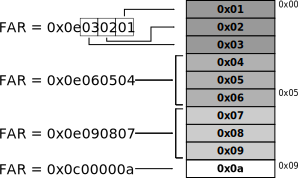
\includegraphics[scale=1]{fig/multiple-spi}}
  \caption{Effects of FAR writes}
  \label{fig:multiple-spi}
\end{figure}

%------------------------------------------------------------------------------
\end{appendices}

%==============================================================================
% Bibliography
%==============================================================================
\pagebreak
\bibliographystyle{ieeetr}
\bibliography{wb_xil_multiboot}

\end{document}
